\textbf{Seats}
\begin{enumerate}
    \item 10 mins: Intro slides \par
    \item 25 mins: Finish Example 5.4.2 \par
    \textbf{Check piazza}
    \item 32 mins: Start example 5.5.1 \par
    \item 45 mins: Finish Example 5.5.1 \par
    \textbf{Check piazza}
    \item 50 mins: Wrap up
\end{enumerate}
\textbf{Seats}

\newcommand{\vect}[1]{\underline{\mathbf{#1}}}

\vspace{5mm} 

\textbf{Example 5.4.2} \par

Since $z=1+i$ is a solution, and the polynomial has real coefficients, $\bar{z}=1-i$ is also a solution. Therefore
\begin{align*}
    (z-1-i)(z-1+i) = z^2-2z+2
\end{align*}
is a factor of the cubic. It follows that
\begin{align*}
    z^3 + 2z^2 - 6z + 8 = (z^2-2z+2)(z-a)
\end{align*}
where $a$ is the real solution. Comparing constant terms $-2a = 8$, so $a=-4$. So, the solutions are
\begin{align*}
    z = 1+i \; , \; 1-i \; , \; {\rm and} \; -4 \,
\end{align*}

\vspace{10mm}
\textbf{Example 5.5.1} \par
    
The first locus is $2 {\rm Re}(z) + {\rm Im}(z - (1+2i)) = 10$, which becomes
\begin{align*}
	2x + y-2 &= 10 \\
	y = 12 - 2x
\end{align*}
So, straight line with gradient -2 that starts at (0,12).

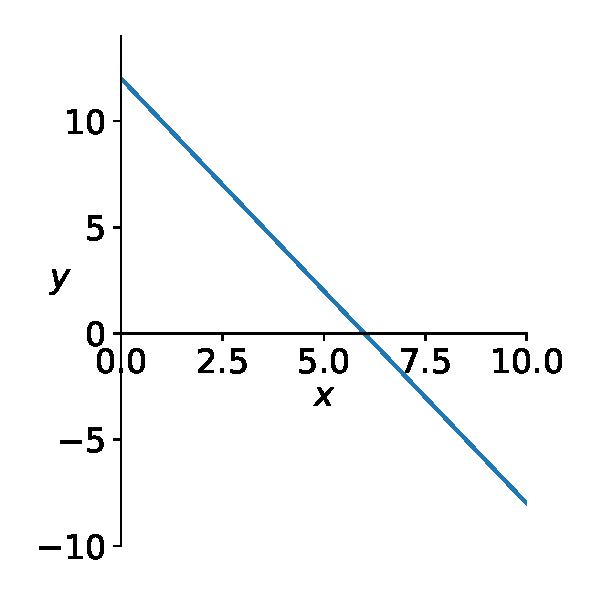
\includegraphics[width=0.4\textwidth]{Figures/ex_551a.pdf}

The second locus is $|z| = {\rm Re}(z+2)$, which becomes
\begin{align*}
	\sqrt{x^2+y^2} &= (x+2) \\
	x^2 + y^2 &= (x+2)^2 \\
	x^2 + y^2 &= x^2 + 4x + 4\\
	y^2 &= 4x + 4
\end{align*}
This can be rearranged to $4x = y^2-4$ so $x = (y-2)(y+2)/4$.

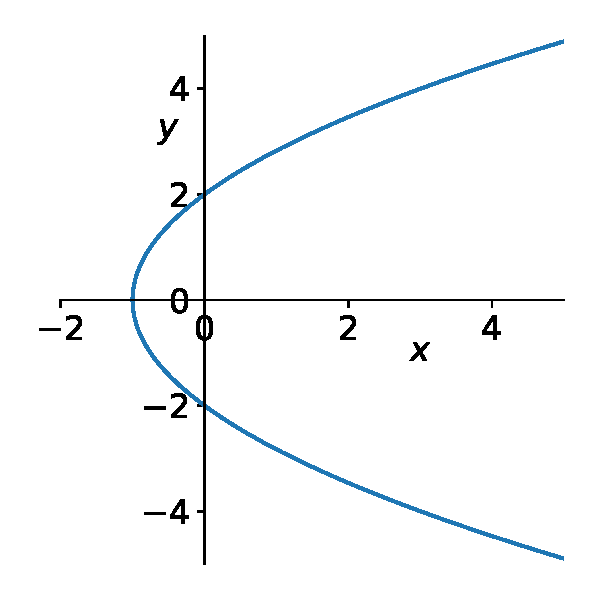
\includegraphics[width=0.4\textwidth]{Figures/ex_551b.pdf}
